\chapter{Lattice Basics}
In this section we want to present the basic concepts of lattice field theory, which has developed to a highly sophisticated research area in the last decades especially in the regime of QCD. This approach to field theory is not only of major concern for performing numerical calculations. It even provides a natural attempt to regularization, which makes it also an interesting topic for theorists in the field of gauge theories.
\section{Discretizing the Lattice}
\label{sec: disc_lat}
A computer is not able to deal with continuous variables, since already a continuous real interval can contain an infinite amount of points, but a computer only has limited memory. Hence we need to limit the amount of points that we consider to make calculations. Since all the target space coordinates\footnote{which represent the fields in our two-dimensional QFT} depend on the worldsheet coordinates $\tau$ and $\sigma$, it seems natural to discretize the worldsheet map. We therefore introduce a lattice spacing $a$ and the lattice size in spacial direction $L$ and in time direction $T$. Following the remarks in \cite{gattringer2009quantum} we define the two-dimensional lattice $\mathit{\Lambda}$ to be
\begin{equation}
\mathit{\Lambda} = \left\lbrace \left(n_{0},n_{1}\right) \vert n_{0}=0,1,\ldots,(T-1) \; ; \;  n_{1}=0,1,\ldots,(L-1) \right\rbrace.
\end{equation}
With that we can express the worldsheet coordinates with the lattice coordinates
\begin{equation}
\left( \tau,\sigma \right) = \left( an_{0},an_{1} \right).
\end{equation}
% ------------------------------------------------
%     tikz graphic lattice mapping
% ------------------------------------------------
\begin{figure}[!ht]
	\centering
\begin{tikzpicture}[scale=1.8]
%flat grid
\draw (-1,-1) rectangle (1,1);
\path (-1,-1) -- node[below]{$\tau$} (1,-1);
\path (-1,-1) -- node[left]{$\sigma$} (-1,1);
\draw [step=0.5cm,dashed] (-1,-1) grid (1,1);
\path (0,0) circle (0.6pt) node[below=2pt, fill=white]{\tiny $(an_{0},an_{1})$};
\foreach \x in {-1,-0.5,...,1}{
	\foreach \y in {-1,-0.5,...,1}{
		\fill (\x,\y) circle (0.6pt);
	}
}
\draw (3,-0.5) -- (4,1);
\draw (5,-0.5) -- (6,1);
\draw (3,-0.5) .. controls +(1,0.7) and +(-1,-0.5) .. (5,-0.5);
\draw (4,1) .. controls +(1,0.7) and +(-1,-0.5) .. (6,1);
\def\v{0.25}
\def\w{0.375}
\def\r{0.58}
\def\z{0.6}
\foreach \x in {1,2,3}
\draw [dashed] (3+\x*\v,-0.5+\x*\w) .. controls +(1,0.7) and +(-1,-0.5) .. (5+\x*\v,-0.5+\x*\w);
%
\draw[dashed] (3.47+\r*\v,-0.5+\r*\w) -- (4.47+\z*\v,1+\z*\w);
\def\a{0.05}
\def\b{0.04}
\draw[dashed] (4.1+\a*\v,-0.5+\a*\w) -- (5.1+\b*\v,1+\b*\w);
\def\c{-0.25}
\def\d{-0.29}
\draw[dashed] (4.7+\c*\v,-0.5+\c*\w) -- (5.7+\d*\v,1+\d*\w);
\draw [->] (1.3,0) .. controls (1.8,0.8) and (2.3,0.8) .. (3,0.8);
\end{tikzpicture}
\caption{Mapping of the worldsheet grid into target space.}
\end{figure}
%
%
%
And since the lattice spacing is overall constant we can abbreviatly refer to a field $\mathit{\Phi}$ in the theory as a function of the lattice variables $\mathit{\Phi}(n_{0},n_{1})$. We now further want to discretize differential operators and integrals. The differentiation can be discretized in various ways inspired by its mathematical definition via differential quotients. To see additionally which order of error is introduced compared to the exact derivative, we examine the \names{Taylor} expansion of a real function $f(x)$ with a small offset $\epsilon$
\begin{equation}
f(x\pm \epsilon) = f(x) \pm \epsilon f'(x) +\dfrac{\epsilon^{2}}{2}f''(x) \pm \dfrac{\epsilon^{3}}{6}f'''(x) + \ldots.
\end{equation}
Now we can define a forward derivative as the finite difference
\begin{equation}
\dfrac{f(x+\epsilon)-f(x)}{\epsilon} = f'(x) + \mathcal{O}(\epsilon)
\end{equation}
and in the same way also a backward derivative by using the $f(x-\epsilon)$ term. Combining both leads to the symmetric derivative with an error of higher order in $\epsilon$
\begin{equation}
\dfrac{f(x-\epsilon)-f(x+\epsilon)}{2 \epsilon} = f'(x) + \mathcal{O}(\epsilon^{2}).
\end{equation}
It is more convenient to use the symmetric finite difference, because the error introduced by the finite lattice spacing is hereby reduced by one order.  By adding additional terms of $f(x\pm 2 \epsilon)$ it is possible to get a finite difference derivative which is exact up to an order of $\mathcal{O}(\epsilon^{3})$ and so on. Depending on the demanded accuracy one is able to regulate the introduced error via this method. With $\epsilon$ being our lattice spacing $a$ we find the derivative of our fields at $n=\left(n_{0}, n_{1} \right)$ to be\footnote{\noindent With $\widehat{\del }_{\alpha}$ beeing the symmetric finite difference in $\alpha$-direction. We also define the forward and backward finite difference respectively by
\begin{equation*}
\vec{\del}_{\alpha}\mathit{\Phi}(n)=\dfrac{\mathit{\Phi}(n+\hat{\alpha})-\mathit{\Phi}(n)}{a} \quad \text{and} \quad
\cev{\del}_{\alpha}\mathit{\Phi}(n)=\dfrac{\mathit{\Phi}(n)-\mathit{\Phi}(n-\hat{\alpha})}{a}.
\end{equation*}
}
%
%
\begin{equation}
\del_{\alpha} \mathit{\Phi}(\tau,\sigma) = \widehat{\del }_{\alpha}\mathit{\Phi}(n) + \mathcal{O}(a^{2}) \equiv \dfrac{\mathit{\Phi}(n-\hat{\alpha})-\mathit{\Phi}(n+\hat{\alpha})}{2a} + \mathcal{O}(a^{2}),
\end{equation}
\begin{equation}
\text{with} \qquad \del_{\alpha}\mathit{\Phi}(\tau,\sigma) \equiv \dfrac{\del \mathit{\Phi}(\tau,\sigma)}{\del \sigma_{\alpha}}, \qquad \sigma_{\alpha}=(\tau,\sigma), \qquad \alpha=0,1
\end{equation}
and where $\hat{\alpha}$ is the unit vector in $\alpha$-direction. For the integration over the worldsheet coordinates we replace the integral by a finite sum over all lattice points
\begin{equation}
\int \dd\tau \dd\sigma \longrightarrow a^{2}\sum\limits_{n \in \mathit{\Lambda}}.
\end{equation}
%
%
For a better visualization it is more convenient to use an abbreviated notation. In the following we will denote $\phi \equiv \phi(n)$ as a field which depends on the lattice coordinates $n$. The same is true for an operator $M\equiv M(m,n)$. A shorter expression of a matrix-vector like product is given by
%
%
\begin{equation}
\phi^{T}M \psi \equiv \sum\limits_{m,n \in \mathit{\Lambda}} \phi(m) M(m,n) \psi(n)\, .
\end{equation}
%
%
To implement the previous relation on a computer as an actual matrix-vector product it is necessary to map the grid index $n=(n_{0},n_{1})$ to a lexicographic vector index
%
%
\begin{equation}
l (n)= Ln_{0} + n_{1} \qquad \text{with} \qquad  l=0,1,\ldots,(V-1),\quad V=LT,
\end{equation}
%
%
so that the according fields $\phi_{l(n)}\equiv \phi(n)$ are actual vectors. For the finite differences derivatives we also need  to know the neighboring relations. So if we want to move on the grid in direction $\pm \hat{\alpha}$, which lexicographic index corresponds to this movement? These relations are implemented into a \textit{next neighbor} function (nb) which also takes into account the boundary conditions (toroidal in our case) and returns the corresponding vector index
%
%
\begin{equation}
l_{\pm\hat{\alpha}} = \text{nb}\,(l,\pm\hat{\alpha}).
\end{equation}
%
%
We now want to define a symmetric finite difference without the factor $1/a$ for the lexicographic notation by
%
%
\begin{equation}
\bar{\Delta}_{\alpha} \phi_{l} \equiv \frac{1}{2}\left(\phi_{l_{+\hat{\alpha}}}-\phi_{l_{-\hat{\alpha}}}\right).
\end{equation}
%
%
In consequence we can write $\bar{\Delta}_{\alpha}$ as a $V\times V$ matrix
%
%
\begin{equation}
\left(\bar{\Delta}_{\alpha}\right)_{lp} = \frac{\delta_{l_{+\hat{\alpha}},p} - \delta_{l_{-\hat{\alpha}},p}}{2}.
\end{equation}
%
%
For other than periodic boundary conditions some of the signs have to be flipped according to the relation (\ref{eq: boundary_cond}).
In the same way we can define forward and backward finite differences by
%
%
\begin{align}
\left(\Delta_{\alpha}\right)_{lp} &= \delta_{l_{+\hat{\alpha}},p}-\delta_{l,p},  &
\left(\Delta^{*}_{\alpha}\right)_{lp} &= \delta_{l,p}-\delta_{l_{-\hat{\alpha}},p}.
\end{align}
We will come back to this notation in \autoref{sec: towards_lat}. For now on we will presume using the grid notation for the further studies.
%
%
%
%
%
%
%- - - - - - -  Bosons and fermions on the lattice
%
%
%
%
%
%
\section{Bosons and Fermions on the Lattice}
\subsection{Bosonic Propagator}
In the examined theory bosons and fermions are both scalar fields of either real, or complex \names{Grassmann} type. The equations of motion of bosons are given by the \names{Klein-Gordon} equation, which contains only second derivatives. To discretize the second derivative we define the corresponding finite difference operator simply by applying a forward and a backward finite difference
\begin{align}
{\widehat{\del}_\alpha}^{\,2}\mathit{\Phi}(n) = \cev{\del}_{\alpha}\vec{\del}_{\alpha}\mathit{\Phi}(n) = \dfrac{\mathit{\Phi}(n+\hat{\alpha})-2\mathit{\Phi}(n)+\mathit{\Phi}(n-\hat{\alpha})}{a^{2}}.
\label{second deriv}
\end{align}
In a Lagrangian we would find the differential operator enclosed by the fields, for instance like
\begin{equation}
\mathit{\Phi}(n)\big({\widehat{\del}_\alpha}^{\,2}\mathit{\Phi}\big)(n) = \sum\limits_{m \in \mathit{\Lambda}} \mathit{\Phi}(n) {\widehat{\del}_\alpha}^{\,2}(n,m) \mathit{\Phi}(m),
\end{equation}
where we use (\ref{second deriv}) to define
\begin{equation}
{\widehat{\del}_\alpha}^{\,2}(n,m) \equiv	\dfrac{\delta_{m,n+\hat{\alpha}}-2\delta_{m,n}+\delta_{m,n-\hat{\alpha}}}{a^{2}}.
\end{equation}
To investigate the behaviour of bosons under the discretization we are interested in the propagator, which is the inverse of the differential operator in momentum space. We therefore perform a discrete \names{Fourier} transform, which is discussed in Appendix \ref{app: disc_ft}. Both indices $m$ and $n$ transform independently and in order to perform a unitary similarity transformation the second index is \names{Fourier} transformed using the complex conjugated phase \cite{gattringer2009quantum}
\begin{align}
{\widetilde{\del}_\alpha}^{\,2}(p,q) &= \dfrac{1}{\vert \mathit{\Lambda}\vert} \sum\limits_{m,n \in \mathit{\Lambda}} \mathrm{e}^{-iq\cdot na} \, {\widehat{\del}_\alpha}^{\,2}(n,m) \, \mathrm{e}^{i p\cdot ma} \notag \\
&= \dfrac{1}{\vert \mathit{\Lambda}\vert}\sum\limits_{n \in \mathit{\Lambda}} \mathrm{e}^{-i (q-p)\cdot na} \dfrac{1}{a^{2}} \left[ \mathrm{e}^{i p_{\alpha} a} -2 +\mathrm{e}^{-i p_{\alpha}a} \right] \\
&= \delta(p-q) \, {\widetilde{\del}_\alpha}^{\,2}(p), \notag
\end{align}
 where the \names{Fourier} transform of the second derivative is defined by
 \begin{equation}
 {\widetilde{\del}_\alpha}^{\,2}(p) \equiv -\dfrac{4}{a^2}\sin^{2}\left(\dfrac{p_{\alpha}a}{2}\right).
 \label{momentum laplace}
 \end{equation}
 The \names{Euclidean} \names{Klein-Gordon} operator $\widetilde{D}(p)$ in momentum space with particle mass $m$ reads
 \begin{equation}
 \widetilde{D}(p) = m^2 + \sum\limits_{\alpha=0}^{1} {\widetilde{\del}_\alpha}^{\,2}(p) .
 \end{equation}
And so we find the propagator simply by inverting the previous relation. Of special interest is the massless case, where we want to investigate the continuum limit
\begin{equation}
\left.\widetilde{D}^{-1}(p)\right\vert_{m=0}=\dfrac{1}{-\dfrac{4}{a^2} \sum\limits_{\alpha=0}^{1} \sin^{2}\left(\dfrac{p_{\alpha}a}{2}\right) } \xrightarrow{a \rightarrow 0} -\dfrac{1}{p^2}.
\end{equation}
This is precisely what we expected for the \names{Euclidean} propagator in the continuum. Since we have $p_{\alpha}\in \left(-\tfrac{\pi}{a},\tfrac{\pi}{a}\right]$, there are no additional poles within the sine function other than the physical one at $p=(0,0)$.
%
%
%
%  FERMION DOUBLING
%
%
\subsection{Fermionic Propagator and the Doubling Problem}
\label{sec: ferm_doubling}
In the case of fermions the equations of motion in 4-dimensional QFT are given by the Dirac equation, which is a linearisation of the \names{Klein-Gordon} equation and only contains first derivatives. To not explicitly break existing symmetries, we have to go with the symmetric derivative in this case. Now we can follow the exact same steps as for the bosonic case to investigate the continuum limit of a \names{Dirac} like operator in our 2-dimensional space time. As mentioned we start from the symmetric finite difference
\begin{equation}
\widehat{\del}_{\alpha}(m,n) \equiv \dfrac{\delta_{m,n+\hat{\alpha}}-\delta_{m,n-\hat{\alpha}}}{2a}
\end{equation}
and proceed with the \names{Fourier} transform
\begin{align}
\widetilde{\del}_{\alpha}(p,q) &= \dfrac{1}{\vert \mathit{\Lambda}\vert} \sum\limits_{m,n \in \mathit{\Lambda}} \mathrm{e}^{-i q\cdot na} \, {\widehat{\del}_\alpha}(n,m) \, \mathrm{e}^{i p\cdot ma} \\
&= \dfrac{1}{\vert \mathit{\Lambda}\vert}\sum\limits_{n \in \mathit{\Lambda}} \mathrm{e}^{- i (q-p)\cdot na} \left[ \dfrac{\mathrm{e}^{i p_{\alpha}a}-\mathrm{e}^{- i p_{\alpha}a}}{2a} \right] \\
&= \delta(p-q)\, \widetilde{\del}_{\alpha}(p),
\end{align}
here we are left with the following differential operator in momentum space
\begin{equation}
\widetilde{\del}_{\alpha}(p) \equiv \dfrac{i}{a} \sin (p_{\alpha}a).
\label{eq: naive_first_dev}
\end{equation}
To construct an \names{Euclidean} \names{Dirac} like operator in two dimensions we use the first two \names{Pauli} matrices\footnote{\[\gamma_{0}=\sigma_{1}=\left( \begin{array}{cc}
0 & 1 \\
1 & 0
\end{array}  \right) \qquad \gamma_{1}=\sigma_{2}=\left( \begin{array}{cc}
0 & -i \\
i & 0
\end{array}  \right) \]}
%
%
\begin{equation}
\widetilde{D}_{D}(p)=  m\mathds{1} + \sum\limits_{\alpha=0}^{1} \gamma_{\alpha}\, \widetilde{\del}_{\alpha}(p)  =m\mathds{1} + \dfrac{i}{a}\sum\limits_{\alpha=0}^{1} \gamma_{\alpha} \sin (p_{\alpha}a)\,.
\end{equation}
The inverse propagator follows from the properties of the \names{Pauli} matrices to be
\begin{equation}
\widetilde{D}_{D}^{-1}(p) = \dfrac{m\mathds{1} - \tfrac{i}{a}\sum_{\alpha=0}^{1} \gamma_{\alpha} \sin (p_{\alpha}a)}{ m^2 + a^{-2}\sum_{\alpha=0}^{1} \sin^2 (p_{\alpha}a)  }.
\end{equation}
Once more we want to study the continuum limit of the propagator for the massless case and find by setting $m=0$
\begin{equation}
\left.\widetilde{D}_{D}^{-1}(p)\right\vert_{m=0} =  \dfrac{- \tfrac{i}{a}\sum_{\alpha=0}^{1} \gamma_{\alpha} \sin (p_{\alpha}a)}{ a^{-2}\sum_{\alpha=0}^{1} \sin^2 (p_{\alpha}a)  } \xrightarrow{a \rightarrow 0} \dfrac{-i \sum_{\alpha=0}^{1} \gamma_{\alpha} p_{\alpha} }{p^2}.
\end{equation}
Here again the propagator has the correct naive continuum limit but this time we face another problem. Since again $p_{\alpha}$ is in the domain $\left(-\tfrac{\pi}{a},\tfrac{\pi}{a}\right]$, there occur three other non-physical poles within the sine function at $p=(0,\pi/a)$, $p=(\pi/a,0)$ and $p=(\pi/a,\pi/a)$. As a result in the numerical simulation it seems that there are in this case three additional fermions, which emerge only from the method of discretization and are  non-physical. This is obviously leading to distorted calculations and needs to be circumvented. That particular problem is known as fermion doubling and has been investigated extensively by \names{Wilson}, who introduced a possible solution.  He suggested to add a term proportional to the discretized \names{Laplace} operator\cite{montvay_lattice}, which is known as a \names{Wilson} term. We can express it in momentum space with the help of (\ref{momentum laplace}) and find\footnote{using the identity
\begin{align*}
\cos(2x)&=\cos^{2}(x) -\sin^{2}(x) \\
\Leftrightarrow\quad \sin^{2}(x) &= \tfrac{1}{2}\left(1-\cos(2x)\right)
\end{align*}
}
%
%
\begin{equation}
W(p)\equiv -\mathds{1}\dfrac{a}{2} \sum\limits_{\alpha=0}^{1} {\widetilde{\del}_\alpha}^{\,2}(p) = \mathds{1}\dfrac{1}{a}\sum\limits_{\alpha=0}^{1}\left( 1- \cos(p_{\alpha}a)\right).
\label{eq: wilson_op}
\end{equation}
Since the \names{Laplace} operator is of order $\mathcal{O}(a^{0})$, we see that the \names{Wilson} term vanishes in the continuum limit. It also vanishes for $p_{\alpha}=0$ and therefore gives no contribution to the physical pole of the theory. If we now invert the new \names{Dirac-Wilson} operator
\begin{equation}
\widetilde{D}_{W}(p) \equiv \widetilde{D}_{D}(p) + W(p),
\end{equation}
we find the new massless momentum space propagator
\begin{equation}
\left. \widetilde{D}_{W}^{-1}\right\vert_{m=0} = \dfrac{\mathds{1}\tfrac{1}{a}\sum_{\alpha=0}^{1}\left( 1- \cos(p_{\alpha}a)\right) - \tfrac{i}{a}\sum_{\alpha=0}^{1}\gamma_{\alpha} \sin(p_{\alpha}a) }{\left(\tfrac{1}{a}\sum_{\alpha=0}^{1}\left( 1- \cos(p_{\alpha}a)\right)\right)^{2} + \tfrac{1}{a^2}\sum_{\alpha=0}^{1}\sin^2(p_{\alpha}a) }.
\end{equation}
Here we can convince ourselves, that there are no more additional poles in the domain of $p_{\alpha}$, since for the points where $p_{\alpha}=\pi/a$ the denominator does not vanish like before. Actually for these points the \names{Wilson}-term behaves like an additional mass term that is growing infinitely in the continuum limit and consequently decouples from the theory.
%
%
%
%-------------------------------------------------------------------------------------------
%
%                 Monte Carlo Methods
%
%-------------------------------------------------------------------------------------------
%
%
%
\section{Monte Carlo Methods}
Now after we know, how to discretize differential operators and act with them on bosonic and fermionic quantities, we are able to build a discretized Lagrangian as well. But what we really need is a method to perform the calculation of observables in the path integral formalism. In QFT in the continuum we calculate the expectation value of an observable $O$ via \cite{peskin}
\begin{equation}
\left\langle O \right\rangle = \dfrac{1}{Z} \int \mathcal{D} \mathit{\phi}\, O(\mathit{\phi})\exp\left(-S\left[\mathit{\phi}\right]\right),
\label{PI_continuum}
\end{equation}
where $S$ is the \names{Euclidean} action depending on the collection of fields $\phi$ and $Z$ is the partition function
\begin{equation}
Z =  \int \mathcal{D} \mathit{\phi}\, \exp\left(-S\left[\mathit{\phi}\right]\right).
\end{equation}
In fact there is no rigorous mathematical definition for the path integral in the continuum. It is motivated from a discretized measure, which is then somehow said to be made continuus. This step is considered ill defined by most mathematicians, but since we stay on a discretized lattice, the path integral measure $\mathcal{D} \mathit{\phi}$ can be perfectly well defined and is represented by
\begin{equation}
\mathcal{D} \mathit{\phi} = \prod\limits_{n \in \mathit{\Lambda}} \dd \phi(n).
\end{equation}
This means, that for every lattice point a multidimensional integral needs to be calculated. Even for small lattices this task becomes tortuous and soon even supercomputers would not be able to do that calculation in reasonable time. Out of this reason other methods of calculation have been considered. The most favoured one is a statistical method going under the name of Monte Carlo simulation. With this type of calculation it is possible to obtain good statistical approximations of high-dimensional integrals in reasonable time. At this point we want to study some details of the Monte Carlo methods used in the scope of this thesis.
%
%
\subsection{Monte Carlo Integration}
The easiest way to understand the idea behind any form of calculation with Monte Carlo methods is via the Monte Carlo integration. Suppose we want to calculate the following multi-dimensional integral
\begin{equation}
I=\int_{\Omega} f(x) \,\dd x,
\end{equation}
where $\Omega\subset \mathbb{R}^{n}$ is a compact integration domain. Then probability theory tells us \cite{mc_methods}, that we can approximate the integral $I$ with a set of random numbers $\left\lbrace \overline{x}_{1},\ldots,\overline{x}_{N}\right\rbrace$ uniformly distributed on $\Omega$ with
\begin{equation}
I_{N}=V \dfrac{1}{N}\sum\limits_{i=1}^{N} f(\overline{x}_{i}).
\end{equation}
Hereby $V=\int_{\Omega}\dd x$ denotes the integration volume. One can show that $I_{N}$ approximates $I$ up to an error of order $\mathcal{O}(1/\sqrt{N})$ and the law of large numbers tells us, that $\lim\limits_{N\to\infty}I_{N}=I$. One can also write for the expectation value $\langle f \rangle$ of $f$, that
\begin{equation}
\langle f \rangle = \lim\limits_{N\to\infty}\dfrac{1}{N}\sum\limits_{i=1}^{N} f(\overline{x}_{i}) = \dfrac{\int_{\Omega} f(x) \,\dd x}{\int_{\Omega}\dd x}.
\end{equation}
An instructive example is to calculate the value of $\pi$ with the 2D-integral $I=\int_{\Omega}H(x,y)\,\dd x\dd y$ over the domain $\Omega=[-1,1]\times [-1,1]$ with the function
\begin{equation}
H(x,y)=\left\lbrace \begin{array}{l}
1\quad \text{if}\quad x^2+y^2\leq 1 \\
0\quad \text{else}.
\end{array} \right.
\end{equation}
Analytically we know that $I$ corresponds to the area of the unit circle and has the value $I=\pi$. With the volume being $V=4$ we can find an estimate
\begin{equation}
\pi \approx \dfrac{4}{N} \sum\limits^{N}_{i=1}H(\overline{x}_{i}).
\end{equation}
This means that we can estimate the value of $\pi/4$ by counting the number of points lying within the circle (see figure \ref{pi_est}) and dividing by the total number of points.
%-----------------------------
%    figure pi estimate
%-----------------------------
\begin{figure}[!ht]
\begin{center}
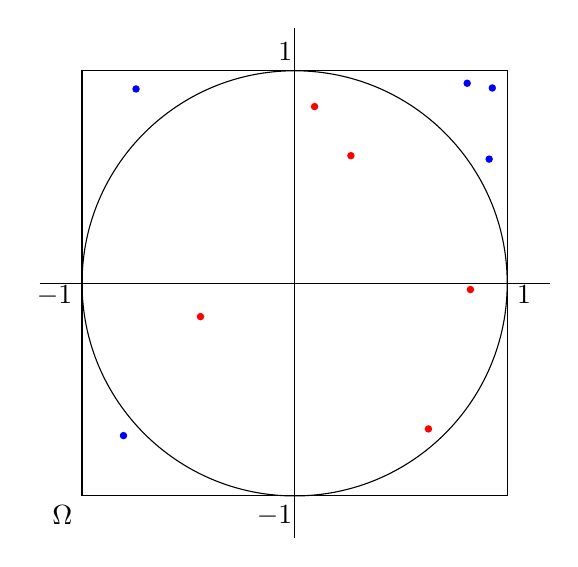
\begin{tikzpicture}[scale=2.7]
 \draw (-1.2,0) -- (1.2,0);
 \draw (0,-1.2) -- (0,1.2);
 \draw (0,0) circle (1cm);
\draw (-1,-1) node [anchor= north east] {$\Omega$} rectangle (1,1);

\draw (-1 cm,-1pt) -- (-1 cm,1pt) node[anchor=north east] {$-1$};
\draw (1 cm,-1pt) -- (1 cm,1pt) node[anchor=north west] {$1$};

\draw (-1pt,1 cm) -- (1pt,1 cm) node[anchor=south east] {$1$};
\draw (-1pt,-1 cm) -- (1pt,-1 cm) node[anchor=north east] {$-1$};

%points within
\fill [red] (0.6294 ,  -0.6848) circle (0.5 pt);
\fill [red] (0.8268 ,  -0.0292) circle (0.5 pt);
\fill [red] (0.2647 ,   0.6006) circle (0.5 pt);
\fill [red] (-0.4430 ,  -0.1565) circle (0.5 pt);
\fill [red] (0.0938,    0.8315) circle (0.5 pt);
%outer points
\fill [blue] (0.8116 ,   0.9412) circle (0.5 pt);
\fill [blue] (-0.7460 ,   0.9143) circle (0.5 pt);
\fill [blue] (-0.8049  , -0.7162) circle (0.5 pt);
\fill [blue] ( 0.9150  ,  0.5844) circle (0.5 pt);
\fill [blue] (0.9298  ,  0.9190) circle (0.5 pt);
\end{tikzpicture}
\end{center}
\caption{Graphic of random numbers uniform in $\Omega$. $\pi/4$ can be estimated by the number of red points within the circle divided by total number of points.}
\label{pi_est}
\end{figure}
%
%
%
%
%
\subsection{Importance Sampling and Markov Chains}
More generally one can estimate integrals over a function $f(x)$ multiplied with a certain weight function $\rho(x)$ in the same way. We can write for the expectation value
\begin{equation}
\langle f \rangle_{\rho} \equiv \dfrac{\int _{\Omega} f(x)\rho(x)\,\dd x}{\int _{\Omega} \rho(x)\,\dd x} = \lim\limits_{N\to\infty}\dfrac{1}{N}\sum\limits_{i=1}^{N} f(\overline{x}_{i}).
\end{equation}
But in this case the random numbers $\overline{x}_{i}$ need to be distributed through the weight function $\rho(x)$. For this to be possible $\rho(x)$ needs to be a valid probability density function.
Comparing with (\ref{PI_continuum}) we can convince ourselves, that this is the case for the \names{Euclidean} path integral. We can exploit this fact to make our calculation more efficient. In principle one could go with the simple Monte Carlo integration scheme, but since our integration domain is no compact interval but the $\mathbb{R}^{n}$, we would produce lots of configurations that would give no contribution to the path integral due to the weight factor and therefore introduce a large error. So if we produce random configurations distributed through a probability density given by the weight factor, we would generate mostly configurations with a non vanishing contribution and the statistical error will be reduced. This procedure is called importance sampling. But to do the importance sampling one needs to be able to produce random configurations according to the given probability density. Since the action appearing in this probability density is in general a very complicated function, this task becomes highly non trivial and there usually is no way to directly transform uniformly distributed random configurations into the favoured form. To make this more explicit, consider the one dimensional integral with normalized probability density function \cite{rothe}
%
%
\begin{equation}
\langle f \rangle_{\rho} = \int \limits_{a}^{b}f(x)\rho(x) \,\dd x\, , \quad \int\limits_{a}^{b} \rho(x)\, \dd x=1.
\end{equation}
%
%
The distribution function $P(x)$ is given by
\begin{equation}
P(x) = \int\limits_{a}^{x} \rho(t)\, \dd t .
\end{equation}
%
%
If we perform the substitution
%
%
\begin{equation}
y(x) \equiv P(x), \quad \text{with} \quad \rho(x) = P'(x)=y'(x), \quad y \in [0,1],
\end{equation}
%
%
we are left with
%
%
\begin{equation}
\langle f \rangle_{\rho} = \int \limits_{a}^{b}f(x) y'(x) \,\dd x = \int\limits_{0}^{1} f\left(x\left(y\right)\right) \dd y,
\end{equation}
%
%
where $x(y)=P^{-1}(y)$. So if we generate uniformly distributed random numbers $\overline{y}$ and use $\overline{x}=P^{-1}(\overline{y})$, which is now distributed according to $\rho(x)$, we can write
%
%
\begin{equation}
\langle f \rangle_{\rho} = \lim_{N \to \infty} \dfrac{1}{N} \sum\limits_{i=1}^{N} f(\overline{x}_{i}).
\end{equation}
%
%
For this to be true $P(x)$ needs to be strongly increasing and globally invertible. Extended to the higher-dimensional problem of path integrals this demand is met very unlikely, as said before.

To circumvent this issue one uses a statistical model called \names{Markov} chain to obtain configurations that are distributed according to the \names{Boltzmann} factor of the path integral. The idea is to start from an arbitrary configuration and generate a new one from the previous configuration via a pseudo random number generation process. Thereby new configurations are generated in a stochastic sequence that eventually follows an equilibrium distribution $P(\mathit{\phi})$ \cite{gattringer2009quantum}. The configurations in the chain can be numbered by an index, the so called Monte Carlo time
%
%
\begin{equation}
\mathit{\phi}_{0} \rightarrow \mathit{\phi}_{1} \rightarrow \ldots \rightarrow \mathit{\phi}_{N_{\text{th}}} \rightarrow \ldots \; .
\end{equation}
%
%
The first configurations up to an index $N_{\text{th}}$ should not be used for measurements since they are most certainly not properly distributed. The process needs a specific amount of time to reach its equilibrium distribution. Therefore this period is called equilibration or thermalization phase.
A \names{Markov} process is characterized by a conditional transition probability $T(\mathit{\phi}' \vert \mathit{\phi})$ to move from a configuration $\mathit{\phi}$ to $\mathit{\phi}'$. This probability depends only on the configurations $\mathit{\phi}$ and $\mathit{\phi}'$ and not any previous ones. It obeys the properties
%
%
\begin{equation}
0 \leq T(\mathit{\phi}' \vert \mathit{\phi}) \leq 1, \quad \sum\limits_{\mathit{\phi}} T(\mathit{\phi}' \vert \mathit{\phi}) =1.
\label{trans_prob}
\end{equation}
%
%
An important restriction is that the process must not get stuck at any configuration. It must always be possible to move between two specified configurations within a finite Monte Carlo time. This can be realised if the transition probability is strictly positive between all states which is called strong ergodicity. Furthermore the probability to move to $\mathit{\phi}'$ from any other state must be the same as to leave $\mathit{\phi}'$ to any other state which can be condensed to the following balance equation
%
%
\begin{equation}
\sum\limits_{\mathit{\phi}} T(\mathit{\phi}' \vert \mathit{\phi}) P(\mathit{\phi}) = \sum\limits_{\mathit{\phi}} T(\mathit{\phi} \vert \mathit{\phi}') P(\mathit{\phi}').
\end{equation}
%
%
A special solution to this equation will be obtained if one assumes that the equation holds for every term of the sum
%
%
\begin{equation}
T(\mathit{\phi}' \vert \mathit{\phi}) P(\mathit{\phi}) = T(\mathit{\phi} \vert \mathit{\phi}') P(\mathit{\phi}').
\end{equation}
%
%
This condition is called detailed balance and is used by most algorithms generating \names{Markov} chains.
%
%
%
%
%- - - - - - - - - - - - - - - - - - - - - - - -
%
\subsection{Fermions on the Lattice and the Hybrid Monte Carlo Algorithm}
\label{sec: hmc_alg}
%
%
There are many possible algorithms to generate field configurations. The choice is depending on the structure of the problem at hand. For the here presented case the algorithm of choice is called rational hybrid Monte Carlo (RHCM). The basic reason to use this algorithm is the presence of fermions in a specific manner. It is in general complicated to deal with fermions in numerical simulations due to the anti commuting properties of \names{Grassmann} variables. An efficient procedure is to integrate out fermions via \names{Grassmann} integration, presented in Appendix \ref{sec: grassmann_analysis}, which results in our case in the Pfaffian of a fermionic operator $M[\phi]$ depending on the bosonic fields $\phi$. We now want to include the Pfaffian as a probability weight factor in the process of generating \names{Markov} chain configurations. To act as a probability weight factor, $\text{Pf}\,M$ must be real and nonnegative. If we consider this to be the case for the moment, we can write
%
%
\begin{equation}
\pf M = (\det M)^{\frac{1}{2}} = \left( \det MM^{\dagger}\right)^{\frac{1}{4}} .
\label{pfaff}
\end{equation}
%
%
In general one could have to deal with an arbitrary fraction $\alpha$ in the exponent on the right side of (\ref{pfaff}). If we restrict $\pf M$ to be also nonzero and therefore entirely positive using that $MM^{\dagger}$ is positive definite, one can rewrite the determinant as a bosonic path integral with pseudofermions $\eta$
%
%
\begin{equation}
\left( \det MM^{\dagger}\right)^{\alpha} = \dfrac{1}{\det \left(MM^{\dagger}\right)^{-\alpha}} \sim \int \mathcal{D}\eta\,\mathcal{D}\eta^{\dagger}\; e^{-\eta^{\dagger}(MM^{\dagger})^{-\alpha}\eta}\, .
\end{equation}
%
%
Since there is an inversion included, the operator in the exponent is highly nonlocal in the bosonic fields $\phi$. So even a small change in the fields could cause a large difference in the weight factor. Ergo one needs an algorithm that ensures that the generated configurations are part of the contributing regime of the weight factor. In a case like that it proved efficient to use a hybrid Monte Carlo (HMC) algorithm when $\alpha=1$, which uses \names{Hamiltonian} dynamics trajectories along some fictitious time to generate new configurations. For non-integer $\alpha$ one can use a rational approximation of $\left(MM^{\dagger}\right)^{-\alpha}$. Combined with the HMC this is called the rational hybrid Monte Carlo (RHMC) algorithm.\\
%
At this point we want to introduce the HMC algorithm which has been proposed in \cite{hmc}. A more detailed explanation is presented in \cite{gattringer2009quantum,montvay_lattice} which serves as a guideline for the following. The HMC is referred to as hybrid because it combines a molecular dynamic (MD) evolution with random noise patterns to simulate quantum fluctuations, an additional \names{Metropolis} acceptance step lets it result into an exact MC algorithm. The field update is  separated into two phases. Pseudofermions are updated first with an exact heat bath, while the bosons are kept constant. Therefore, a configuration $\xi$ is generated from a \names{Gaussian} distribution $P(\xi) \sim e^{-\xi^{\dagger}\xi}$ and we set $\eta = M\xi$.\\
In the second phase a molecular dynamic evolution is used to update the bosonic fields while the pseudofermions are kept constant.  We can now think of the effective action $S_{\rm eff}[\phi]= S_{\rm B}[\phi] + \eta^{\dagger}(MM^{\dagger})^{-1}\eta$ as only dependent on the bosonic fields $\phi$. Now for each field $\phi_{i}$ a conjugate momentum $\pi_{i}$ is introduced and we expand the path integral with $\int \mathcal{D}\pi\, \exp(-1/2 \;\pi^{2})$ to obtain
%
%
\begin{equation}
\langle O \rangle = \dfrac{\int \mathcal{D}\phi \mathcal{D}\eta \mathcal{D}\pi\;  O(\phi) \,e^{-H[\phi,\pi]}}{\int \mathcal{D}\phi \mathcal{D}\eta \mathcal{D}\pi\;  e^{-H[\phi,\pi]}},
\end{equation}
where we have introduced the \names{Hamiltonian}
%
%
\begin{equation}
H[\phi,\pi] = \frac{1}{2}\pi^{2} + S_{\rm eff}[\phi]\, , \quad \pi^{2}=\sum\limits_{i}\sum\limits_{n\in \mathit{\Lambda}}\pi_{i}^{2}(n)\, .
\end{equation}
%
%
The evolution of the fields follows according to the classical equations of motion along a fictitious MC time $\tau$
%
%
\begin{align}
\dot{\pi}_{i} &=-\frac{\del H}{\del \phi_{i}} = -\frac{\del S_{\rm eff}}{\del \phi_{i}} \notag \\
\dot{\phi}_{i} &= \frac{\del H}{\del \pi_{i}} = \pi_{i}
\label{ham_eom}
\end{align}
%
%
A numerical implementation of (\ref{ham_eom}) introduces a discrete step size $\epsilon \equiv \delta	\tau$ and errors of order $\mathcal{O}(\epsilon^{2})$. An additional \names{Metropolis} acceptance step can correct these errors. First the momenta $\pi$ are randomly generated from a \names{Gaussian} distribution $P_{\rm G}(\pi)=\exp(-1/2\,\pi^{2})$. Then a numerical integration scheme is used to change the configuration $\lbrace \phi,\pi \rbrace$ along a discretized trajectory in phase space to the new point $\lbrace \phi',\pi' \rbrace$. The transition probability $T_{\rm MD}(\phi',\pi' \vert \phi,\pi)$ of the MD evolution depends on the integration scheme. The latter needs to be reversible and area preserving for the algorithm to obey detailed balance. Thus, a \textit{leapfrog integration} scheme  is used. For one trajectory the fields $\phi$ are evolved in $n$ steps of length $\epsilon$. The momenta start with half a step of length $\epsilon / 2$, then $(n-1)$ full steps are performed and again a half-step. The first half-step is given by
%
%
\begin{align}
\pi_{i}(\tfrac{\epsilon}{2}) &= \pi_{i}(0) - \frac{\del S_{\rm eff}(\phi(0))}{\del \phi_{i}}\frac{\epsilon}{2}, \notag \\
\phi_{i}(\epsilon) &= \phi_{i}(0) + \pi_{i}(\tfrac{\epsilon}{2}) \epsilon\, .
\end{align}
%
%
The next steps for $j=1,\ldots,n-1$ are
%
%
\begin{align}
\pi_{i}\left(\left(j+\tfrac{1}{2}\right)\epsilon\right) &= \pi_{i}\left(\left(j-\tfrac{1}{2}\right)\epsilon\right) - \frac{\del S_{\rm eff}(\phi(j\epsilon))}{\del \phi_{i}}\epsilon \notag \\
\phi_{i}\left(\left(j+1\right)\epsilon\right) &= \phi^{i}\left(j\epsilon\right) + \pi_{i}\left(\left(j+\tfrac{1}{2}\right)\epsilon\right) \epsilon\, .
\end{align}
%
%
With the last half-step we arrive at the final momentum
%
%
\begin{equation}
\pi_{i}(n\epsilon) = \pi_{i}\left(\left(n+\tfrac{1}{2}\right)\epsilon\right) - \frac{\del S_{\rm eff}(\phi(n\epsilon))}{\del \phi_{i}}\frac{\epsilon}{2}\, .
\end{equation}
%
%
With an additional \names{Metropolis} acceptance step
%
%
\begin{equation}
T_{\rm A}(\phi',\pi' \vert \phi,\pi) = \min(1, \exp ( H[\phi,\pi] - H[\phi',\pi'] )
\end{equation}
%
%
the total transition probability to move from $\phi$ to $\phi'$ is given by
%
%
\begin{equation}
T(\phi'\vert\phi) = \int \mathcal{D}\pi' \mathcal{D}\pi\; T_{\rm A}(\phi',\pi' \vert \phi,\pi) T_{\rm MD}(\phi',\pi' \vert \phi,\pi) P_{\rm G}(\pi)\, .
\end{equation}
%
%
This has been proved to obey detailed balance in \cite{hmc}. Concluding one can summarize the HMC algorithm in the following steps:
%
%
\begin{itemize}
\item \textbf{Pseudofermions}\\
Generate the pseudofermion field $\eta = M\xi$, where $\xi$ is distributed according to $\exp(-\xi^{\dagger}\xi)$.
%
%
\item \textbf{Conjugate fields}\\
For an initial boson configuration $\phi^{(0)}$ generate $\pi^{(0)}$ according to the \names{Gaussian} distribution $\exp(-\tfrac{1}{2}\pi^{2})$.
%
%
\item \textbf{Initial step}\\
$\pi_{i}^{(\frac{1}{2})} = \pi_{i}^{(0)} - \frac{\epsilon}{2}F_{i}\left[\phi\right] \Big\vert_{\phi^{(0)}} \,.$
%
%
\item \textbf{Intermediate steps}\\
Full steps for $j=1,\ldots,n-1$\\[0.2cm]
$\phi_{i}^{(j)} = \phi_{i}^{(j-1)} + \pi_{i}^{(j-\frac{1}{2})}\;, \qquad
\pi_{i}^{(j+\frac{1}{2})} = \pi_{i}^{(j-\frac{1}{2})} -\epsilon  F_{i}\left[\phi\right] \Big\vert_{\phi^{(j)}}\, .
$
%
%
\item \textbf{Final step}\\
$\phi_{i}'=\phi_{i}^{(n)}= \phi_{i}^{(n-1)} + \pi_{i}^{(n-\frac{1}{2})}\;, \quad
\pi_{i}' = \pi_{i}^{(n)} = \pi_{i}^{(n-\frac{1}{2})} - \frac{\epsilon}{2}  F_{i}\left[\phi\right] \Big\vert_{\phi^{(n)}}\,.$
%
%
\item \textbf{Monte Carlo step}\\
Accept new configuration $\phi'$ if a random number $r \in [0,1)$ is smaller than
\[\exp\left(\frac{1}{2}\left(\pi^{2}-\pi'^{2}\right) + S_{\rm B}[\phi]-S_{\rm B}[\phi'] +\xi^{\dagger}\xi - \eta^{\dagger}\left(M'M'^{\dagger}\right)^{-1} \eta \right)\, .  \]
\end{itemize}
%
%
Here we used $\phi_{i}^{(j)}\equiv \phi_{i}(j\epsilon)$ and the driving forces are denoted by
\begin{equation}
F_{i}[\phi] = \frac{\del }{\del \phi_{i}}\left[ S_{\rm B}\left[\phi\right] + \eta^{\dagger}\left(MM^{\dagger}\right)^{-1}\eta \right]\,.
\end{equation}
%
%
%
%
% - - - - - - - - - -   sign problem  - - - - - - - - - -
%
%
%
%
\subsection{Numerical sign problems}\label{sec: sign_prob}
As discussed previously we want to calculate expectation values of observables $O(\phi)$, depending on bosonic fields $\phi$ which are distributed according to a certain probability weight function $\rho(\phi)$
%
%
\begin{equation}
\left\langle O \right\rangle_{\rho} = \frac{\int \mathcal{D}\phi\; O(\phi)\rho(\phi)}{\int \mathcal{D}\phi\; \rho(\phi)}.
\end{equation}
%
%
The feasibility of calculations like that via Monte Carlo methods is only guaranteed if the weight function $\rho(\phi)$ is non-negative. In the process of dealing with fermions it is sometimes necessary to introduce bosonic auxiliary fields by a \names{Hubbard-Stratonovich} (HS)  transformation\footnote{See Appendix \ref{sec: HS_trafo} for futher details on the HS transformation.} which might lead to a complex phase in the weight function. For fluctuations of this phase that are very close to the purely real spectrum, this can be corrected by a reweighting procedure. If nonetheless the phase is distributed on the whole complex spectrum where the reweighting tends to fail, then one is talking of a \textit{sign problem}. There are several approaches to fix this issue but none of them works as a general method to cure the sign problem.
